\chapter{Obiettivi della tesi}
\label{capitolo3}
\thispagestyle{empty}

L'obiettivo di questa tesi è quello di illustrare le modifiche, le aggiunte ed i cambiamenti effettuati al software di LIS per permettere un integrazione dei ricevitori di allarme in maniera più veloce e standard, una seconda parte della tesi complementare alla prima si focalizza invece sulla telegestione del delle centrali di allarme. Marginalmente tratteremo la videosorveglianza ed altri aspetti più pratici che riguardano la gestione di un allarme.
\section{La situazione iniziale}
Al nostro arrivo in LIS la situazione che si presentava era poco chiara e non ben definita. Gli operatori di centrale che gestivano gli allarmi utilizzavano un software denominato \emph{E-Pro}. Questo programma è un adattamento di un programma utilizzato da Cobra SPA per la gestione degli allarmi provenienti da veicoli ed è stato adattato  negli anni alla gestione degli impianti fissi.\\
Questo software è un formato da un insieme di moduli alcuni scritti in C ed altri in Java, la parte che riguarda la ricezione degli allarmi il loro immagazzinamento nel database e la logica che gestisce il comportamento da intraprendere per la loro gestione è implementato in una serie di moduli scritti in C; questi moduli sono chiamati:
\begin{itemize}
	\item cp220\_3
	\item cp220\_4
	\item MTSfe\_fissi
\end{itemize}
Questi tre moduli si occupano della ricezione degli allarmi dai vettori PSTN e GPRS/GSM per fare questo utilizzano dei ricevitori fisici chiamati
\begin{description}
	\item[System III:] si occupa della ricezione degli allarmi sul vettore PSTN tramite protocollo Contact ID.
	\item[OHLan:] questo ricevitore è un PC fisico collegato in LAN sul quale è installato un software della UTC Fire \& Security che si occupa della ricezione tramite protocollo proprietario degli allarmi provenienti dalle centrali UTC.
	\item[Modem GSM:] più di un modem GSM è collegato ad una porta multiseriale connessa nella rete locale questi modem permettono la ricezione degli allarmi tramite vettore GSM e GPRS.
\end{description}
Per quanto riguarda la parte Java essa si occupa dell'interazione con l'operatore e quindi il compito di questi moduli è quello di prelevare gli allarmi dal database e mostrarli all'operatore, inoltre, questi moduli si occupano di tenere traccia di tutte le azioni eseguite dall'operatore. Infine, questa parte è strutturata in modo da garantire la multiutenza, infatti, questi moduli sono scritti in Java EE e sono eseguiti su di un server JBoss in modo da permettere l'esecuzione di più sessioni contemporaneamente.
\begin{figure}
\centering
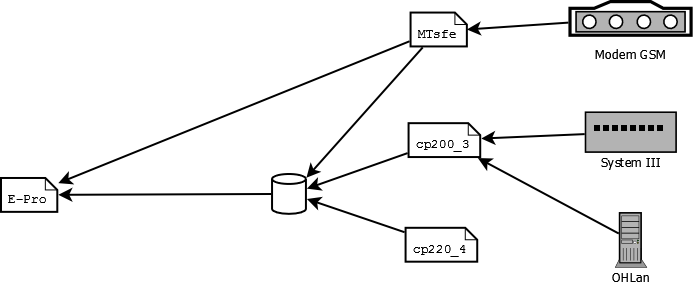
\includegraphics[width=0.7\linewidth]{pictures/struttura.png}
\caption{Schema dei moduli applicativi di LIS}\label{img:struttura}
\end{figure}
\subsection{cp220\_3}
Il \emph{cp220\_3} ha la funzione di leggere e trasformare gli allarmi provenienti dai sistemi di ricezione come il \emph{System III} o lo \emph{OHLan} e di immagazzinarli in un database non prima di averli trasformati in un formato interpretabile dall'E-Pro. questo formato è derivato direttamente dal Contact ID il prevedere diversi campi
\begin{center}
	\texttt{ACCT MT QXYZ GG CCC S}
\end{center}
dove i diversi campi indicano:
\begin{description}
	\item[ACCT:] è un identificativo assegnato al cliente
	\item[MT:] è un numero che indica il tipo di messaggio, se esso è nuovo oppure una ritrasmissione.
	\item[XYZ:] è un codice che indica il tipo di evento che è avvenuto
	\item[Q:] un numero che può essere 1 o 3 ed indica se l'evento trasmesso è rispettivamente iniziato o finito.
	\item[GG:] è il numero che identifica la partizione nella quale è stato generato l'allarme
	\item[CCC:] è un numero che identifica il sensore o zona che ha generato l'allarme.
	\item[S:] valore di checksum per il controllo degli errori
\end{description}
Il \texttt{cp220\_3} utilizza i campi ACCT, XYZ, Q, GG, CCC insieme al timestamp nel quale arriva il messagio e li inserisce in una tabella del database dal quale poi saranno prelevati ed inviati all'operatore.\\
Oltre a questa funzione il modulo all'arrivo di ogni messaggio aggiorna un campo in una tabella chiamata \emph{Ricevitori} per controllare periodicamente lo stato in vita dei ricevitori e la loro connessione con il modulo in questione.\\
Questo modulo è il più interessante per noi in quanto è quello che permette la ricezione degli allarmi e quindi sarà oggetto di una più approfondita analisi.
\subsection{cp220\_4}
Questo modulo si occupa della logica della gestione degli allarmi per capire meglio il funzionamento di questo modulo facciamo un esempio e consideriamo un 
\subsection{MTSfe}
\subsection{E-Pro}
\section{Obiettivi della tesi}
\subsection{Integrazione di nuovi protocolli in minor tempo}
\subsection{Strutturazione del software}
\subsection{Telegestione}
\subsection{Utilizzo di nuovi vettori di comunicazione}
\section{Problematiche legate al software preesistente}


